\subsection{Dalvik Virtual Machine} \label{subsection:android-dalvik}
%START TEXT INPUT
This is my real text! Rest might be copied or not be checked!
%START TEXT INPUT

Flow what is dalvik, what is different to java, what is dex (build process), VGL \url{http://newandroidbook.com/files/ArtOfDalvik.pdf}\newline

%
The applications for Android are written using the Java programming language.

stack abstraction is the Dalvik Virtual Machine (DVM)\newline
DVM is highly tailored to work according to the specifications of the Android platform\newline
optimized for a slower CPU in comparison with a stationary machine andworks with relatively little RAM memory (• limited processor speed
• limited RAM
• no swap space
• battery powered
• diverse set of devices
• sandboxed application runtime)\cite{ehringerDalvik}\newline
DVM is register-based, differing from the standard Java Virtual Machine (JVM) which is stack-based, register-based architectures require fewer executed instructions than stack-based architectures, register-based code is approximately 25 percent larger than the stack-based, the increase in the instructions fetching time is negligible: 1.07 percent extra real machine loads\cite{ehringerDalvik}\newline
the Android OS has no swap space imposing that the virtual machine works without swap. Finally, mobile devices are powered by a battery thus the DVM is optimized to be as energy preserving as possible, Except being highly efficient, the DVM is also designed to be replicated quickly because each application runs within a “sandbox”: a context containing its own instance of the virtual machine assigned a unique Unix user ID\newline

wie der build process funktioniert wird später gesondert beschrieben, hier sagen wir einfach das ergebnis ist die dex datei\newline

\cite{kovachevaMaster} \cite{ehringerDalvik}
%

%
DVM is
- Customized optimized JVM based on Apache Harmony,
- Not fully J2SE or J2ME compatible -see- Java compiles into DEX code -see- 16-bit opcodes and Register, rather than stack-based\newline
History, Dalvík was introduced along with Android, created by Created by Dan Bornstein, Named after an Icelandic town, 2.2 brought current just in time compilation (ERKLÄREN)\newline
Dalvik vs Java
- Dalvík is a virtual machine implementation, Based on Apache Harmony, Borrows heavily from Java
- Brings significant improvements over Java, in particular J2ME, Virtual Machine architecture is optimized for memory sharing, Reference counts/bitmaps stored separately from objects, Dalvik VM startup is optimized through Zygote
- Java .class files are further compiled into DEX.\newline
Overview creating APK
\begin{figure}[h]
    \centering
    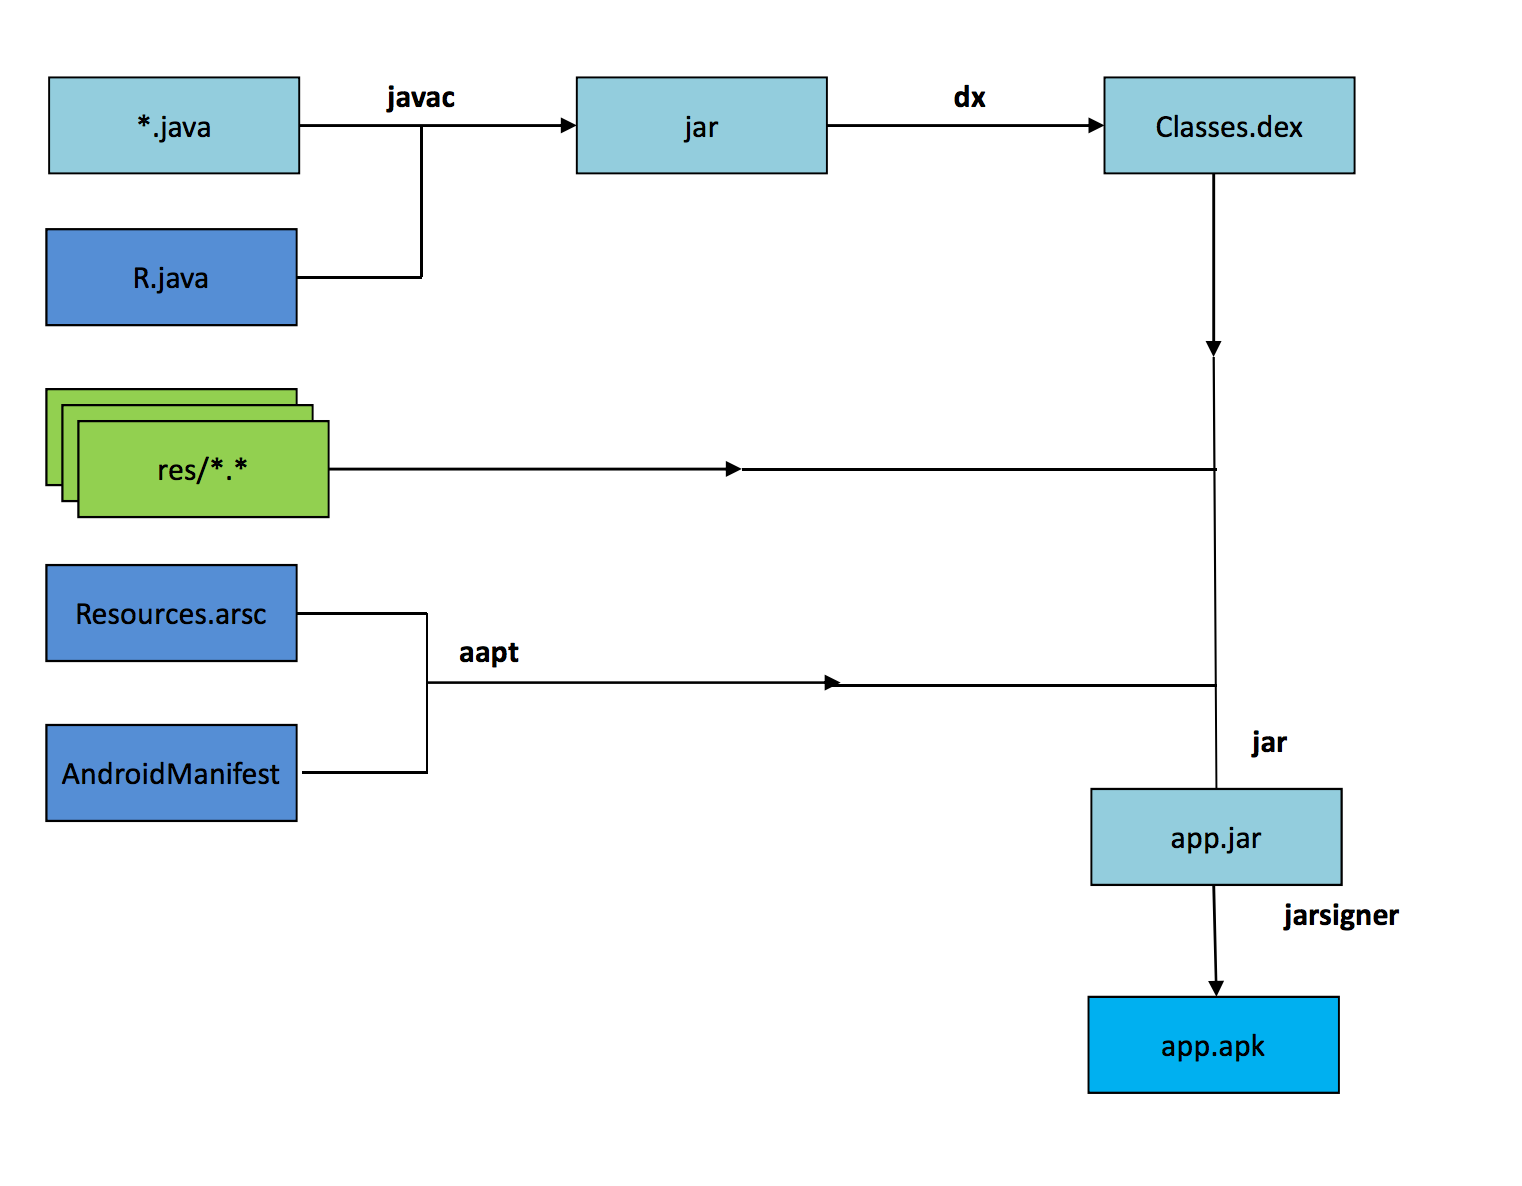
\includegraphics[width=0.8\textwidth]{data/apk.png}
    \caption{Awesome Image}
    \label{fig:awesome_image}
\end{figure}
unterschied zu java und dann auf dex?\newline
\cite{andevconDalvikART}
%



AUFBAU/HERKUNFT DALVIK MACHIEN\newline
difference to JVM -see- JVM is a stack based machine whereas DVM is register based -see- warum, vorteile/nachteile, hisotrie\newline
developed for Android to be more efficient and smaller due to the limited resources on mobile devices -see- quelle\newline

unterschied \url{http://newandroidbook.com/files/Andevcon-DEX.pdf}\newline
